\section{Orientation of a regular surface}
\begin{question}
    Consider \(\mathbb{S}^2\) with spherical parametrization, are following two
    parametrizations the same?
    \begin{itemize}
        \item \((\vphi,\theta)\longmapsto(\sin\vphi\cos\theta,\sin\vphi\sin\theta,
            \cos\vphi)\)
        \item \((\theta,\vphi)\longmapsto(\sin\vphi\cos\theta,\sin\vphi\sin\theta,
            \cos\vphi)\)
    \end{itemize}
\end{question}

The answer is NO\@! They give different normal directions which decide ``inside'' and
``outside'' of \(\mathbb{S}^2\).

\noindent\underline{\bfseries Recall:} \(\mathbb{R}^2\) is orientable. It has two
orientations. Given a basis \(\{e_1,e_2\}\), let
\begin{align*}
    J_{+}=\Bigl\{E_{+}=\{e_1^+,e_2^+\}&:E_{+}\text{ has same orientation as }E.\\
    &\text{ \ie\ }\begin{bmatrix}
        e_1^+\\ e_2^+
    \end{bmatrix}=\underbrace{\begin{bmatrix}
        a_{11} & a_{12} \\
        a_{21} & a_{22}
    \end{bmatrix}}_{A_{+}}\begin{bmatrix}
        e_1 \\ e_2
    \end{bmatrix}
    \text{ and }\det A_{+}>0\Bigr\};
\end{align*}
\begin{align*}
    J_{-}=\Bigl\{E_{-}=\{e_1^-,e_2^-\}&:E_{-}\text{ has same orientation as }E.\\
    &\text{ \ie\ }\begin{bmatrix}
        e_1^-\\ e_2^-
    \end{bmatrix}
    =A_{-}\begin{bmatrix}
        e_1 \\ e_2
    \end{bmatrix}
    \text{ and }\det A_{-}>0\Bigr\}.
\end{align*}
Then either \(J_{+}\) or \(J_{-}\) gives an orientation of \(\mathbb{R}^2\).

\begin{question}\hfill
\begin{enumerate}[(1)]
    \item Let \(S\) be a regular surface, how can we define orientation?
    \item Are all surfaces orientable?
\end{enumerate}
\end{question}

Assume we have two parametrizations around \(p\):
\begin{align*}
    F&\colon U\to S &&T_p S\cong \mathbb{R}^2=\Span\{F_u,F_v\} \\
    G&\colon V\to S &&T_p S\cong \mathbb{R}^2=\Span\{G_\alpha,G_\beta\}
.\end{align*}
Note near \(p\), \(F(u,v)=G(\alpha,\beta)\implies \) \[
    \begin{bmatrix}
        G_\alpha \\ G_\beta
    \end{bmatrix}=\begin{bmatrix}
        u_\alpha & v_\alpha \\
        u_\beta & v_\beta
    \end{bmatrix}\begin{bmatrix}
        F_u \\ F_v
    \end{bmatrix}
.\] 
\ie\ Two parametrizations \(F\) and \(G\) give the same orientation iff \[
    \left|\pdv{(u,v)}{(\alpha,\beta)}\right|>0
.\] 

\begin{definition}[Orientation of a regular surface]
    We say a regular surface \(S\) is orientable if there exists a coordinate
    chart covering of \(S\), \st\ if a point \(p\) belongs to two charts, then the
    induced basis on \(T_p S\) by the two parametrizations have the same orientation
    in above sense.
\end{definition}

\begin{remark}\hfill
\begin{enumerate}[(1)]
    \item ``Orientation'' is a global intrinsic property. ``Orientability'' is
    essentially reflected by the topology of the surface. In algebraic topology
    course, you'll see that the orientability is determined by the 1st
    Stiefel-Whitney class in \(H^1(M,\mathbb{Z}/2\mathbb{Z})\) for a vector
    bundle on topological manifold \(M\).
    With additional ``smooth'' structure on \(M\), we have more ways to check
    the orientability, for example, \(\exists\) a nowhere vanishing top
    differential form (or say, a volume form).
    \item One of important applications of ``orientation'' in this course (and
    later in Reimann Geometry) is allowing us to define ``integration'' on a regular
    surface.
\end{enumerate}
\end{remark}

\begin{exercise}
    Give a definition of orientation of \(\mathbb{R}^n\) as a vector space.
\end{exercise}

\begin{example}[1]
    \(\mathbb{S}^2\) is orientable.
\end{example}

Consider the stereographic parametrization
\begin{align*}
    \pi_N\colon \mathbb{S}^2\setminus\{N\} &\longrightarrow \mathbb{R}^2 \\
    (x,y,z) &\longmapsto (u,v)=(\frac{x}{1-z},\frac{y}{1-z})
.\end{align*} \[
    \pi_N^{-1}(u,v)=(\frac{2u}{1+u^2+v^2},\frac{2v}{1+u^2+v^2},1-\frac{2}{1+u^2+v^2})
.\] \begin{align*}
    \pi_S\colon \mathbb{S}^2\setminus\{S\} &\longrightarrow \mathbb{R}^2 \\
    (x,y,z) &\longmapsto (\alpha,\beta)=(\frac{y}{1+z},\frac{x}{1+z})
.\end{align*} \[
    \pi_N^{-1}(\alpha,\beta)=(\frac{2\beta}{1+\alpha^2+\beta^2},\frac{2\alpha}
    {1+\alpha^2+\beta^2},\frac{2}{1+\alpha^2+\beta^2}-1)
.\] Clearly \(\mathbb{S}^2=\pi_N^{-1}(U)\cup \pi_S^{-1}(V)\). To see the orientation,
we compute the Jacobian of change form one chart to another. \((u,v)\to (\alpha,\beta
)\). Now \[
    \begin{cases}
        u=\frac{x}{1-z} \\
        v=\frac{y}{1-z}
    \end{cases},\quad
    \begin{cases}
        \alpha=\frac{y}{1+z} \\
        \beta=\frac{x}{1+z}
    \end{cases}
.\] Hence \[
    \begin{cases}
        u\alpha=v\beta \\
        u\beta+v\alpha=1
    \end{cases}\implies \ \ 
    \begin{cases}
        u=\frac{\beta}{\alpha^2+\beta^2} \\
        v=\frac{\alpha}{\alpha^2+\beta^2}
    \end{cases}
.\] Then \[
    \pdv{(u,v)}{(\alpha,\beta)}=\begin{pmatrix}
        -\frac{2\alpha\beta}{(\alpha^2+\beta^2)^2} &
        \frac{\alpha^2-\beta^2}{(\alpha^2+\beta^2)^2} \\
        \frac{\beta^2-\alpha^2}{(\alpha^2+\beta^2)^2} &
        -\frac{2\alpha\beta}{(\alpha^2+\beta^2)^2}
    \end{pmatrix}\implies \det>0
.\] 

\begin{example}[2]
    The graph \((x,y,f(x,y))\) is always orientable.
\end{example}

\noindent\textbullet{} Normal vector field and orientation.

Since in this course, we consider the regular surface \(S\) in \(\mathbb{R}^3\),
at each \(p\in S\), there is a unique tangent plane \(T_p S\), which is a 2 dim
linear subspace of \(\mathbb{R}^3\). Hence we can talk abort the normal vector
field on \(S\). Now we want a ``well-defined'' normal by taking ``unit normal vector
\(\vec{n}\)'' at \(p\).

Let's check \(\vec{n}\) under change of parameter. Let \(F\colon U\to S\) be
a parametrization around \(p\). Then \[
    T_p S=\Span\{F_u,F_v\}\implies\vec{n}_F=\frac{F_u\times F_v}{|F_u\times F_v|}
.\] (Note the cross product here already assigns a direction of \(\vec{n}\)).

If \(G\colon V\to S\) is another parametrization around \(p\). Then \[
    T_p S=\Span\{G_\alpha,G_\beta\},\quad \vec{n}_G=\frac{G_\alpha\times G_\beta}
    {|G_\alpha\times G_\beta|}
.\] Let \(\Phi=G^{-1}\circ F\colon U\cap V\to U\cap V\) be the transition map.
Then \[
    \begin{cases}
        F_u=G_\alpha\alpha_u+G_\beta\beta_u \\
        F_v=G_\alpha\alpha_v+G_\beta\beta_v
    \end{cases}
    \text{\ie\ }
    \begin{pmatrix}
        F_u \\ F_v
    \end{pmatrix}=\begin{pmatrix}
        \alpha_u & \beta_u \\
        \alpha_v & \beta_v
    \end{pmatrix}\begin{pmatrix}
        G_\alpha \\ G_\beta
    \end{pmatrix}
.\]
\(\implies F_u\times F_v=\det(\pdv{(\alpha,\beta)}{(u,v)})G_\alpha\times G_\beta\).
Hence \[
    \vec{n}_F=\sign \det(\pdv{(\alpha,\beta)}{(u,v)})\cdot \vec{n}_G
.\] 

\begin{definition}[Unit normal vector field]
    \(U\subset S\) open subset, a unit normal vector field on \(U\) is a smooth map
    \begin{align*}
        \vec{n}\colon U &\longrightarrow \mathbb{R}^3 \\
        p &\longmapsto \vec{n}_p\text{ (unit normal at }p\text{)}
    .\end{align*}
\end{definition}

\begin{prop}
    A regular surface is orientable \(\iff \) there is a unit normal vector field
    \(\vec{n}\colon S\to \mathbb{R}^3\) defined everywhere on \(S\).
\end{prop}

\begin{remark}
    On an orientable regular surface, the ``unit'' normal vector field has image
    on \(\mathbb{S}^2\), \ie\ there is a smooth map 
    \begin{align*}
        \vec{n}\colon S &\longrightarrow \mathbb{S}^2=\{x^2+y^2+z^2=1\} \\
        p &\longmapsto \vec{n}_p
    .\end{align*}
    This \(\vec{n}\) is called the \emph{Gauss map} of the surface. Later we'll
    see that the differential of \(\vec{n}\) determines how the surface is curved
    in \(\mathbb{R}^3\).
\end{remark}

\begin{proof}
    ``\(\implies \)'': If \(S\) is orientable, then \(\exists\) a coordinate chart
    covering \(\{F_\alpha(U_\alpha)\}_{\alpha\in \Lambda}\) of \(S\),
    (\(F_\alpha\colon U_\alpha\to S,S=\bigcup_{\alpha\in \Lambda}F_\alpha(U_\alpha)
    \)). \st\ on \(U_\alpha\cap U_\beta\neq \emptyset\), \[
        \det(\pdv{(u_\alpha,u_\beta)}{(u_\beta,v_\beta)})>0
    .\] Hence at \(p\in U_\alpha\cap U_\beta\), \[
        \vec{n}_p
        =\frac{F_{u_\alpha}\times F_{v_\alpha}}{|F_{u_\alpha}\times F_{v_\alpha}|}
        =\frac{F_{u_\beta}\times F_{v_\beta}}{|F_{u_\beta}\times F_{v_\beta}|}
    .\] (This guarantees that we can extend the normal vector in on chart to another)
    
    Hence we can well define \(\vec{n}\colon S\to \mathbb{R}^3\). The smoothness of
    \(\vec{n}\) can be checked in local coordinates.

    ``\(\impliedby \)'': Let \(\vec{n}\colon S\to \mathbb{R}^3\) be the unit normal
    vector field defined on \(S\). Let \(\{F_\alpha\colon U_\alpha\to S\}\) be a
    coordinate chart covering of \(S\). Then on each \(F_\alpha(U_\alpha)\), \[
        \vec{n}_\alpha
        =\frac{F_{u_\alpha}\times F_{v_\alpha}}{|F_{u_\alpha}\times F_{v_\alpha}|}
    .\] On \(U_\alpha\cap U_\beta\) at some point \(p\), we have \[
        \frac{F_{u_\alpha}\times F_{v_\alpha}}{|F_{u_\alpha}\times F_{v_\alpha}|}
        =\sign \det(\pdv{(u_\beta,v_\beta)}{(u_\alpha,v_\alpha)})\cdot 
        \frac{F_{u_\beta}\times F_{v_\beta}}{|F_{u_\beta}\times F_{v_\beta}|}
    .\] Since \(\vec{n}_\alpha\) and \(\vec{n}_\beta\) agree at \(p\), we see \[
        \det(\pdv{(u_\beta,v_\beta)}{(u_\alpha,v_\alpha)})>0
    .\] 
\end{proof}

\begin{figure}[htb]
    \centering
    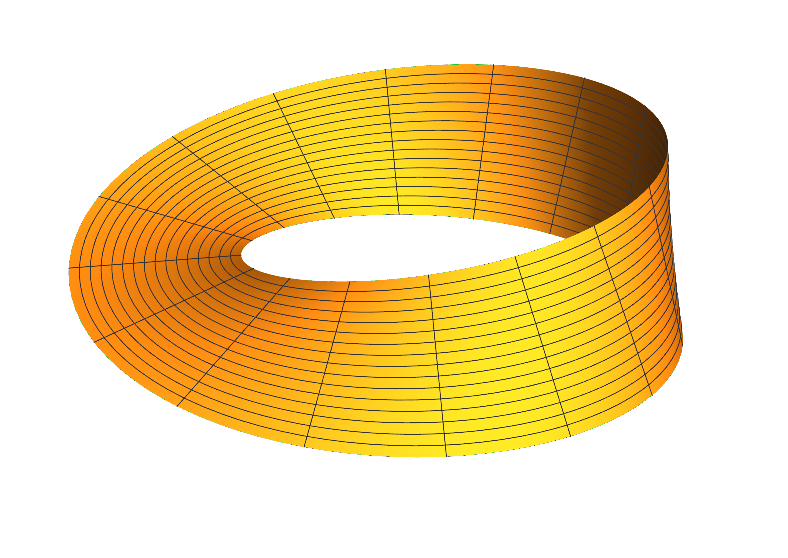
\includegraphics[width=0.5\textwidth]{picture/week6/mobius.pdf}
    \caption{M\"obius strip}\label{fig:mobius}
\end{figure}

\begin{example}[Non-orientated surface]
    M\"obius strip \(M\) (\cref{fig:mobius})
\end{example}

Consider the line segment \(AB\) with equation \(-\frac{1}{2}\le z\le \frac{1}{2},
y=1,x=0\), rotating along a circle \(x^2+y^2=1\). When the center \(c\) moves
about angle \(u\) away from \(y\)-axis, the line \(A'B'\) is in the plane determined
by \(z\)-axis and \(c'\) and the angle between \(A'B'\) and \(z\)-axis is
\(\frac{u}{2}\).

Let \(U=\{(u,v):0<u<2\pi,-\frac{1}{2}<v<\frac{1}{2}\}\), then \[
    F(u,v)=((1-v\sin\frac{u}{2})\sin u,(1-v\sin \frac{u}{2})\cos u,v\cos\frac{u}{2})
.\] This almost covers \(M\), except at \(u=0\). To cover this, we consider
rotation \(AB\) when the center lies on \(x\)-axis. We have parametrization \[
    G(\alpha,\beta)=((1-\beta\sin(\frac{\pi}{4}+\frac{\alpha}{2}))\cos\alpha,
    (1-\beta\sin(\frac{\pi}{4}+\frac{\alpha}{2}))\sin\alpha,
    \beta\cos(\frac{\pi}{4}+\frac{\alpha}{2}))
.\] \[
    V=\{(\alpha,\beta):0<\alpha<2\pi,-\frac{1}{2}<\beta<\frac{1}{2}\}
.\] Now the missing part is on \(u=\frac{\pi}{2}\).

Consider \(F(U)\cap G(V)\), it contains two pieces \[
    W_1=\{F(u,v):0<u<\frac{\pi}{2}\},\quad
    W_2=\{F(u,v):\frac{\pi}{2}<u<2\pi\}
.\] On \(W_1\), \[
    \begin{cases}
        \alpha=u+\frac{3}{2}\pi \\
        \beta=-v
    \end{cases}
    \implies \ \ \left|\pdv{(\alpha,\beta)}{(u,v)}\right|=-1
.\] On \(W_2\), \[
    \begin{cases}
        \alpha=u-\frac{\pi}{2} \\
        \beta=v
    \end{cases}
    \implies \ \ \left|\pdv{(\alpha,\beta)}{(u,v)}\right|=1
.\] No matter how we change parametrization in \(W_1\) or \(W_2\), we can not
guarantee that \(\left|\pdv{(\alpha,\beta)}{(u,v)}\right|\) is positive everywhere.
(\ie\ \(\vec{n}\) has to change sign). Hence \(M\) is non-orientable.

\begin{remark}
    In the following of this course, we only care about orientable surfaces.
    \ie\ surfaces having well-defined unit normal vector field everywhere.
\end{remark}

\section{The first fundamental form on \(S\)}

